\documentclass[11pt]{article}

\usepackage{amsmath,amssymb,mathtools}
\usepackage[margin=1in]{geometry}
\usepackage{enumitem}
\usepackage{xcolor}
\usepackage{microtype}
\usepackage{graphicx}
\usepackage{tikz,float}
\usepackage{subcaption}
\usepackage{amsthm}
\usepackage{hyperref}
\usepackage{array}
\usepackage{pgfplots}

\usetikzlibrary{shapes.geometric, arrows.meta, positioning, calc, decorations.markings}
\tikzset{
	block/.style={rectangle, draw, text width=6em, text centered, rounded corners, minimum height=10mm},
	sum/.style={circle, draw, node distance=1.5cm},
	line/.style={draw, -{Stealth[length=2.5mm, width=1.5mm]}}
}

\usepgfplotslibrary{groupplots}
\pgfplotsset{compat=1.18}

\pgfplotsset{
	myaxes/.style={
		axis lines=middle,
		axis line style={-latex},
		grid=major,
		grid style={gray!15},
		minor grid style={gray!35},
		xlabel style={at={(ticklabel* cs:1)}, anchor=north west},
		ylabel style={at={(ticklabel* cs:1)}, anchor=south east},
		every axis plot/.append style={thick}
	},
	myplotstyle/.style={
		width=14cm,
		height=7cm,
		axis lines=middle,
		axis line style={-Stealth},
		grid=both,
		minor tick num=1,
		major grid style={draw=gray!30},
		minor grid style={draw=gray!15},
		tick label style={font=\small, fill=white, inner sep=1.5pt},
		xlabel={$t$},
		ylabel={$x(t)$},
		xlabel style={anchor=north east, font=\small},
		ylabel style={anchor=south east, font=\small},
		samples=401,
	}
}

\newtheoremstyle{mynote}
{6pt}      % Space above
{6pt}      % Space below
{}          % Body font (normal, not italic)
{}          % Indent amount
{\bfseries} % Theorem head font
{.}         % Punctuation after theorem head
{.5em}      % Space after theorem head
{}          % Theorem head spec
\theoremstyle{mynote}
\newtheorem{definition}{Definition}
\newtheorem{proposition}{Proposition}
\newtheorem{example}{Example}
\newtheorem{remark}{Remark}
\newtheorem{theorem}{Theorem}
\newtheorem{corollary}{Corollary}

\newcommand{\T}{\mathcal{T}}
\newcommand{\R}{\mathbb{R}}
\newcommand{\Z}{\mathbb{Z}}
\newcommand{\C}{\mathbb{C}}
\newcommand{\conv}{\ast}
\newcommand{\dt}{\,\dd t}
\newcommand{\dd}{\mathrm{d}}
\newcommand{\imp}{\delta}
\newcommand{\sinc}[1]{\frac{\sin(\pi #1)}{\pi #1}}


\DeclareMathOperator{\rect}{rect}
\DeclareMathOperator{\Ev}{Ev}
\DeclareMathOperator{\Od}{Od}
\DeclareMathOperator{\sgn}{sgn}
\DeclareMathOperator{\step}{u}
\DeclareMathOperator{\tri}{tri}

\renewcommand{\qedsymbol}{}


\begin{document}
	% Reset figure counter for this lecture
	\renewcommand{\thefigure}{8.\arabic{figure}}
	
	% --- TITLE BLOCK ---
	\thispagestyle{empty}
	\noindent
	\begin{tabular*}{\textwidth}{l @{\extracolsep{\fill}} r}
		\textbf{Signals and Systems} & \textbf{Lecture 8} \\
		\textit{Dr. Ghandi Manasra and Ahmed Rabei} & \textit{Fall 2025} \\
	\end{tabular*}
	\hrule
	\vspace{0.4cm}
	\begin{center}
		\Large\textbf{Lecture 8: Properties of the Continuous-Time Fourier Series}
	\end{center}
	\vspace{0.4cm}
	
	\section*{Reference}
	Oppenheim \& Willsky, \textit{Signals and Systems}, Chapter 3, Section 3.5
	
\section*{Review of Lecture 7}
\begin{itemize}[noitemsep]
	\item Complex exponentials as LTI eigenfunctions
	\item Continuous-Time Fourier Series (CTFS)
	\item Synthesis and analysis equations
	\item Orthogonality and convergence conditions
\end{itemize}
	
\section*{8.1 Introduction}

Last time, we established that complex exponentials are \textbf{eigenfunctions} of LTI systems, meaning that an input $e^{j\omega t}$ produces the output $H(j\omega)e^{j\omega t}$. This motivated the \textbf{Continuous-Time Fourier Series}, which represents a periodic signal $x(t)$ as a sum of harmonically related complex exponentials.

Today, we will examine the properties of this representation. We will explore how operations in the time domain (like shifting or differentiating a signal) affect its frequency-domain representation (the coefficients $a_k$). These properties are not just mathematical curiosities; they are powerful tools that provide deep insight and serve as computational shortcuts.

\section*{8.2 CTFS Properties}
	
	For convenience, we will use the notation $x(t) \stackrel{\mathcal{FS}}{\longleftrightarrow} a_k$ to denote the pairing of a periodic signal with its Fourier series coefficients.
	
	\subsection*{8.2.1 Linearity}
	
	If $x(t) \stackrel{\mathcal{FS}}{\longleftrightarrow} a_k$ and $y(t) \stackrel{\mathcal{FS}}{\longleftrightarrow} b_k$, then:
	\[
	Ax(t) + By(t) \stackrel{\mathcal{FS}}{\longleftrightarrow} Aa_k + Bb_k
	\]

	\subsection*{8.2.2 Time Shifting}
	
	\[
	x(t - t_0) \stackrel{\mathcal{FS}}{\longleftrightarrow} a_k e^{-jk\omega_0 t_0}
	\]
	
	\textbf{Note:} Shifting a signal in time does \textbf{not} change the magnitude of its frequency components, $|a_k|$. It only introduces a \textbf{phase shift}, $-k\omega_0 t_0$, to each coefficient. This phase shift is linear with the harmonic number $k$.
	
	\begin{proof}
		Starting with the synthesis equation for $x(t)$:
		\[
		x(t) = \sum_{k=-\infty}^{\infty} a_k e^{jk\omega_0 t}
		\]
		For the shifted signal $x(t - t_0)$:
		\[
		x(t - t_0) = \sum_{k=-\infty}^{\infty} a_k e^{jk\omega_0 (t - t_0)} = \sum_{k=-\infty}^{\infty} a_k e^{-jk\omega_0 t_0} e^{jk\omega_0 t}
		\]
		Therefore, the coefficients for $x(t - t_0)$ are $a_k e^{-jk\omega_0 t_0}$.
		
	\end{proof}
	
	\subsection*{8.2.3 Time Reversal}
	
	\[
	x(-t) \stackrel{\mathcal{FS}}{\longleftrightarrow} a_{-k}
	\]
	
	\textbf{Note:} Reversing a signal in time also reverses its frequency spectrum.
	
	\textbf{Consequence:}
	\begin{itemize}[noitemsep]
		\item If $x(t)$ is \textbf{even}, then $a_k$ are \textbf{even} ($a_k = a_{-k}$).
		\item If $x(t)$ is \textbf{odd}, then $a_k$ are \textbf{odd} ($a_k = -a_{-k}$).
	\end{itemize}
	
	\subsection*{8.2.4 Conjugation and Symmetry for Real Signals}
	
	For any \textbf{real} signal $x(t)$, the Fourier coefficients are \textbf{conjugate symmetric}:
	\[
	a_k = a_{-k}^*
	\]
	
	\begin{proof}
		For a real signal $x(t)$, we have $x(t) = x^*(t)$. Starting with the definition of $a_k^*$:
		\[
		a_k^* = \left( \frac{1}{T_0} \int_{T_0} x(t)e^{-jk\omega_0 t} \dd t \right)^* = \frac{1}{T_0} \int_{T_0} x^*(t)e^{jk\omega_0 t} \dd t
		\]
		Since $x(t)$ is real, $x^*(t) = x(t)$, so:
		\[
		a_k^* = \frac{1}{T_0} \int_{T_0} x(t)e^{jk\omega_0 t} \dd t = \frac{1}{T_0} \int_{T_0} x(t)e^{-j(-k)\omega_0 t} \dd t = a_{-k}
		\]
		Therefore, $a_k = a_{-k}^*$ for real signals.
	\end{proof}
	
	\textbf{Consequences:}
	\begin{itemize}[noitemsep]
		\item The magnitude is an \textbf{even} function: $|a_k| = |a_{-k}|$.
		\item The phase is an \textbf{odd} function: $\angle a_k = -\angle a_{-k}$.
		\item The DC component $a_0$ is real.
		\item If $x(t)$ is real and even, the coefficients $a_k$ are \textbf{real and even}.
		\item If $x(t)$ is real and odd, the coefficients $a_k$ are \textbf{purely imaginary and odd}.
	\end{itemize}
	
	\begin{remark}
		These are extremely useful. If you are given a real and even signal, you immediately know that you only need to compute the real-valued coefficients $a_k$ for $k \geq 0$, as the rest are determined by symmetry. This can cut the work in half.
	\end{remark}
	
	\subsection*{8.2.5 Parseval's Theorem for Periodic Signals}
	
	This property relates the average power in the time domain to the power in the frequency domain as follows:
	\[
	\frac{1}{T_0} \int_{T_0} |x(t)|^2 \dd t = \sum_{k=-\infty}^{\infty} |a_k|^2
	\]
	The total average power of a signal is the sum of the average powers of all its harmonic components. This shows that the \textbf{average power} is conserved between the time and frequency domains.
	
	The term $|a_k|^2$ is the average power in the $k^{th}$ harmonic. A plot of $|a_k|^2$ versus frequency is called the signal's \textbf{power spectrum}.
	
	\begin{proof}
		Starting with the integral for power:
		\[
		\frac{1}{T_0}\int_{T_0} x(t)x^*(t)\dd t = \frac{1}{T_0}\int_{T_0} x(t) \left( \sum_{k=-\infty}^{\infty} a_k^* e^{-jk\omega_0 t} \right) \dd t
		\]
		Swapping the sum and integral (assuming convergence):
		\[
		= \sum_{k=-\infty}^{\infty} a_k^* \left( \frac{1}{T_0}\int_{T_0} x(t)e^{-jk\omega_0 t} \dd t \right) = \sum_{k=-\infty}^{\infty} a_k^* a_k = \sum_{k=-\infty}^{\infty} |a_k|^2
		\]
		 
	\end{proof}
	
	\subsection*{8.2.6 The Differentiation Property}
	
	\[
	\frac{\dd x(t)}{\dd t} \stackrel{\mathcal{FS}}{\longleftrightarrow} jk\omega_0 a_k
	\]
	
	\textbf{Note:} Differentiation is a \textbf{high-pass} operation. The $jk\omega_0$ factor amplifies the coefficients at higher frequencies (larger $k$) more than those at lower frequencies.
	
	\textbf{Physical Interpretation:} Derivatives measure the rate of change of a signal. Rapid changes (high frequencies) are emphasized, while slow changes (low frequencies) are attenuated. This is why differentiation acts as a high-pass filter - it naturally emphasizes the high-frequency content of signals.
	
	\begin{proof}
		Differentiating the synthesis equation:
		\[
		\frac{\dd x(t)}{\dd t} = \frac{\dd}{\dd t} \sum_{k=-\infty}^{\infty} a_k e^{jk\omega_0 t} = \sum_{k=-\infty}^{\infty} a_k \frac{\dd}{\dd t} e^{jk\omega_0 t} = \sum_{k=-\infty}^{\infty} jk\omega_0 a_k e^{jk\omega_0 t}
		\]
	\end{proof}
	
	\subsection*{8.2.7 Integration Property}
	
	If $x(t) \stackrel{\mathcal{FS}}{\longleftrightarrow} a_k$ and $a_0 = 0$, then:
	\[
	\int_{-\infty}^t x(\tau) \dd\tau \stackrel{\mathcal{FS}}{\longleftrightarrow} \frac{a_k}{jk\omega_0}
	\]
	
	\textbf{Note:} Integration is a \textbf{low-pass} (smoothing) operation. The $\frac{1}{jk\omega_0}$ factor attenuates higher frequencies more than lower frequencies.
	
	\textbf{Condition Explanation:} The condition $a_0 = 0$ (zero average value) is necessary because if it were non-zero, the integral $\int_{-\infty}^t x(\tau) \dd\tau$ would contain a term $a_0 t$, which grows with time and is not periodic. The Fourier Series can only represent periodic signals.
	
	\subsection*{8.2.8 Frequency Shifting (Modulation)}
	
	\[
	x(t) e^{jm\omega_0 t} \stackrel{\mathcal{FS}}{\longleftrightarrow} a_{k-m}
	\]
	
	\textbf{Note:} Multiplying a signal by a complex exponential shifts its entire frequency spectrum. This is the fundamental principle behind radio modulation, where a low-frequency signal (like voice) is shifted to a high-frequency band for transmission.
	
	\section*{8.3 Additional Properties and Relationships}
	
	\subsection*{8.3.1 Multiplication Property}
	
	The multiplication of two periodic signals in the time domain corresponds to convolution of their Fourier series coefficients in the frequency domain:
	\[
	x(t)y(t) \stackrel{\mathcal{FS}}{\longleftrightarrow} (a * b)_k = \sum_{\ell=-\infty}^{\infty} a_\ell b_{k-\ell}
	\]
	
	This property is particularly useful for modulation and mixing operations in communications systems.
	
	\subsection*{8.3.2 Conjugation Property}
	
	For any signal $x(t)$:
	\[
	x^*(t) \stackrel{\mathcal{FS}}{\longleftrightarrow} a_{-k}^*
	\]
	
	This property is useful for analyzing the frequency content of complex signals and for understanding the relationship between positive and negative frequency components.
	
	\subsection*{8.3.3 Time Scaling}
	
	For a time-scaled signal $x(at)$ where $a > 0$:
	\[
	x(at) \stackrel{\mathcal{FS}}{\longleftrightarrow} a_k \text{ with fundamental frequency } a\omega_0
	\]
	
	Time scaling compresses or expands the signal in time, which corresponds to expanding or compressing the frequency spectrum.
	\newpage
	\section*{8.4 Practical Applications of Properties}
	
	\subsection*{8.4.1 Finding the CTFS of a Triangular Wave}
	
	We can use the differentiation property to find the coefficients for a periodic triangular wave, $x(t)$, from the coefficients of a square wave, $g(t)$.
	
	\begin{figure}[H]
		\centering
		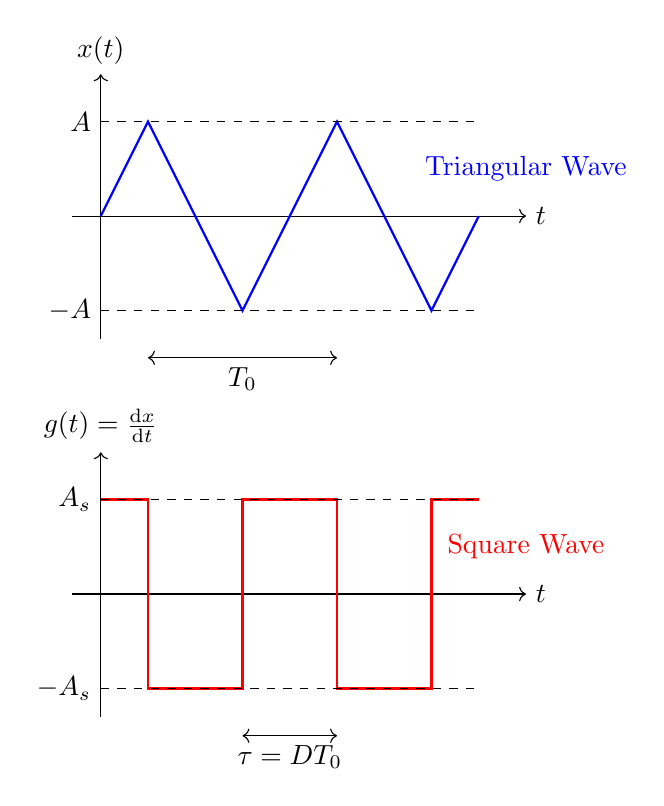
\begin{tikzpicture}[scale=1.2]
	% Triangular wave x(t)
	\begin{scope}[yshift=4cm]
		\draw[->] (-0.3,0) -- (4.5,0) node[right] {$t$};
		\draw[->] (0,-1.3) -- (0,1.5) node[above] {$x(t)$};
		\draw[thick, blue] (0,0) -- (0.5,1) -- (1.5,-1) -- (2.5,1) -- (3.5,-1) -- (4,0);
		\node[blue] at (4.5,0.5) {Triangular Wave};
		\draw[dashed] (0,1) -- (4,1);
		\draw[dashed] (0,-1) -- (4,-1);
		\node[left] at (0,1) {$A$};
		\node[left] at (0,-1) {$-A$};
		\draw[<->] (0.5,-1.5) -- (2.5,-1.5) node[midway,below] {$T_0$};
	\end{scope}
	
	% Square wave g(t) = dx/dt
	\begin{scope}
		\draw[->] (-0.3,0) -- (4.5,0) node[right] {$t$};
		\draw[->] (0,-1.3) -- (0,1.5) node[above] {$g(t) = \frac{\mathrm{d} x}{\mathrm{d} t}$};
		\draw[thick, red] (0,1) -- (0.5,1) -- (0.5,-1) -- (1.5,-1) -- (1.5,1) -- (2.5,1) -- (2.5,-1) -- (3.5,-1) -- (3.5,1) -- (4,1);
		\node[red] at (4.5,0.5) {Square Wave};
		\draw[dashed] (0,1) -- (4,1);
		\draw[dashed] (0,-1) -- (4,-1);
		\node[left] at (0,1) {$A_s$};
		\node[left] at (0,-1) {$-A_s$};
		\draw[<->] (1.5,-1.5) -- (2.5,-1.5) node[midway,below] {$\tau = DT_0$};
	\end{scope}
\end{tikzpicture}

		\caption{Triangular wave and its derivative (square wave)}
		\label{fig:triangular_square_wave}
	\end{figure}
	
	Let $x(t)$ be a triangular wave with period $T_0$ and amplitude $A$. The derivative $g(t) = \frac{\dd x(t)}{\dd t}$ is a square wave with amplitude equal to the slope of the triangular wave (e.g., $4A/T_0$ for a symmetric wave) and coefficients:
	\[
	b_k = \frac{4A}{T_0} D \cdot \text{sinc}(Dk)
	\]
	where $D$ is the duty cycle and $\text{sinc}(x) = \frac{\sin(\pi x)}{\pi x}$.
	

	From the differentiation property: $b_k = jk\omega_0 a_k$
	
	For $k \neq 0$:
	\[
	a_k = \frac{b_k}{jk\omega_0} = \frac{\frac{4A}{T_0} D \cdot \text{sinc}(Dk)}{jk\omega_0} = \frac{4A D}{j2\pi k} \text{sinc}(Dk)
	\]
	
	The DC component $a_0$ is found by inspection (the average value of the triangular wave).
	
	\begin{figure}[H]
		\centering
		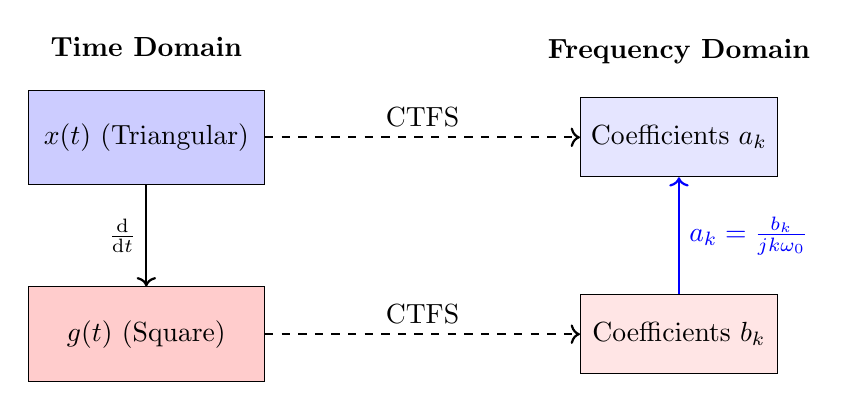
\begin{tikzpicture}[node distance=2.5cm, auto]
    % Nodes
    \node[draw, rectangle, minimum width=3cm, minimum height=1.2cm, fill=blue!20] (xt) {$x(t)$ (Triangular)};
    \node[draw, rectangle, minimum width=3cm, minimum height=1.2cm, fill=red!20, below of=xt] (gt) {$g(t)$ (Square)};
    \node[draw, rectangle, minimum width=2.5cm, minimum height=1cm, fill=blue!10, right=4cm of xt] (ak) {Coefficients $a_k$};
    \node[draw, rectangle, minimum width=2.5cm, minimum height=1cm, fill=red!10, right=4cm of gt] (bk) {Coefficients $b_k$};
    % Arrows
    \draw[->, thick] (xt) -- (gt) node[midway,left] {$\frac{\dd}{\dd t}$};
    \draw[->, thick, dashed] (xt) -- (ak) node[midway,above] {CTFS};
    \draw[->, thick, dashed] (gt) -- (bk) node[midway,above] {CTFS};
    \draw[->, thick, blue] (bk) -- (ak) node[midway,right] {$a_k = \frac{b_k}{jk\omega_0}$};
    % Labels
    \node[above=0.3cm of xt] {\textbf{Time Domain}};
    \node[above=0.3cm of ak] {\textbf{Frequency Domain}};
\end{tikzpicture}

		\caption{The differentiation property relationship showing how time-domain differentiation corresponds to frequency-domain multiplication by $jk\omega_0$.}
		\label{fig:differentiation_property_relationship}
	\end{figure}
	
	\begin{remark}
		\textbf{The smoother a signal is, the faster its Fourier series coefficients decay to zero.}
		
		\begin{itemize}[noitemsep]
			\item \textbf{Square Wave (Discontinuous):} The coefficients $b_k$ decay proportionally to $\frac{1}{k}$.
			\item \textbf{Triangular Wave (Continuous):} The coefficients $a_k$ contain an extra factor of $1/k$ from the integration, so they decay much faster, proportionally to $\frac{1}{k^2}$.
		\end{itemize}
		
		This faster decay means that a smooth signal like a triangular wave can be accurately approximated with fewer sinusoidal harmonics compared to a sharp, discontinuous signal like a square wave.
	\end{remark}
	
	\begin{figure}[H]
		\centering
		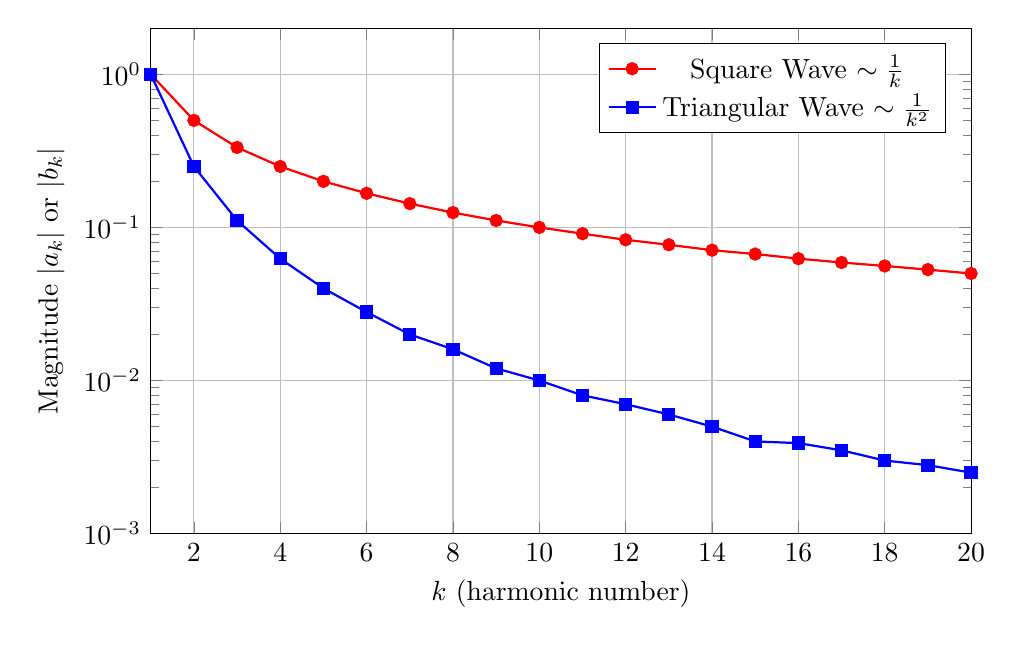
\begin{tikzpicture}
\begin{axis}[
    xlabel={$k$ (harmonic number)},
    ylabel={Magnitude $|a_k|$ or $|b_k|$},
    legend pos=north east,
    grid=major,
    ymode=log,
    xmin=1, xmax=20,
    ymin=0.001, ymax=2,
    width=12cm,
    height=8cm
]
% Square wave: 1/k decay
\addplot[red, thick, mark=*, mark size=2pt] coordinates {
    (1,1) (2,0.5) (3,0.333) (4,0.25) (5,0.2) 
    (6,0.167) (7,0.143) (8,0.125) (9,0.111) (10,0.1)
    (11,0.091) (12,0.083) (13,0.077) (14,0.071) (15,0.067)
    (16,0.0625) (17,0.059) (18,0.056) (19,0.053) (20,0.05)
};
\addlegendentry{Square Wave $\sim \frac{1}{k}$}
% Triangular wave: 1/k^2 decay
\addplot[blue, thick, mark=square*, mark size=2pt] coordinates {
    (1,1) (2,0.25) (3,0.111) (4,0.0625) (5,0.04) 
    (6,0.028) (7,0.02) (8,0.016) (9,0.012) (10,0.01)
    (11,0.008) (12,0.007) (13,0.006) (14,0.005) (15,0.004)
    (16,0.0039) (17,0.0035) (18,0.003) (19,0.0028) (20,0.0025)
};
\addlegendentry{Triangular Wave $\sim \frac{1}{k^2}$}
\end{axis}
\end{tikzpicture}

		\caption{Comparison of Fourier coefficient decay rates}
		\label{fig:coefficient_decay_comparison}
	\end{figure}
	
	\subsection*{8.4.2 Summary of CTFS Properties}
	
	\begin{table}[H]
		\centering
		\begin{tabular}{|l|c|c|}
			\hline
			\textbf{Property} & \textbf{Time Domain} $x(t)$ & \textbf{Frequency Domain} $a_k$ \\
			\hline
			Linearity & $Ax(t) + By(t)$ & $Aa_k + Bb_k$ \\
			\hline
			Time Shifting & $x(t - t_0)$ & $a_k e^{-jk\omega_0 t_0}$ \\
			\hline
			Time Reversal & $x(-t)$ & $a_{-k}$ \\
			\hline
			Conjugation (Real Signals) & $x(t)$ real & $a_k = a_{-k}^*$ \\
			\hline
			Differentiation & $\frac{\dd x(t)}{\dd t}$ & $jk\omega_0 a_k$ \\
			\hline
			Integration & $\int_{-\infty}^t x(\tau) \dd\tau$ & $\frac{a_k}{jk\omega_0}$ (if $a_0 = 0$) \\
			\hline
			Frequency Shifting & $x(t) e^{jm\omega_0 t}$ & $a_{k-m}$ \\
			\hline
			Parseval's Theorem & $\frac{1}{T_0} \int_{T_0} |x(t)|^2 \dd t$ & $\sum_{k=-\infty}^{\infty} |a_k|^2$ \\
			\hline
		\end{tabular}
		\caption{Summary of Continuous-Time Fourier Series Properties}
		\label{tab:ctfs_properties}
	\end{table}
	
	\section*{8.5 Summary and Next Lecture}
	
	As we have demonstrated, the properties of the CTFS form a powerful 'dictionary' for translating operations between the time and frequency domains. These properties provide both computational shortcuts and deep physical insights into how signals behave.
	
	\begin{itemize}[noitemsep]
		\item Time shifting introduces linear phase shifts proportional to frequency
		\item Differentiation acts as a high-pass filter, integration as a low-pass filter
		\item Real signals have conjugate-symmetric coefficients, reducing computation by half
		\item Parseval's relation shows energy conservation between time and frequency domains
		\item Properties provide powerful shortcuts for finding Fourier series coefficients
		\item \textbf{Next time:} We will develop the parallel representation for discrete-time periodic signals: the \textbf{Discrete-Time Fourier Series (DTFS)}. We will see many similarities, but also some critical differences that arise from the discrete nature of time.
	\end{itemize}
	
\end{document}
